\section{Main theorem}

\begin{frame}{Outline}
On a single face we have \( I^X_F\defeq\loopy(\flat_F(X_1)\cdot X_F)\).\\~\\

\onslide<2->{We will show}
\begin{itemize}
\item<3-> how to sum this over faces
\item<4-> that \( X_F \) adds up to zero, by a cancellation argument
\end{itemize}
\onslide<5->{and the theorem \( I^X_{\mathrm{tot}}=\loopy(\flat_\mathrm{tot}) \) will follow.}\\~\\

\onslide<6->{We will \alert{remove the dependency} on \( \mm \), by using our materials in new ways.}
\end{frame}

% \begin{frame}{Angle}
% \begin{columns}
% \begin{column}{0.3\textwidth}
% \begin{tikzpicture}%
  [x={(-0.860769cm, -0.121512cm)},
  y={(0.508996cm, -0.205391cm)},
  z={(-0.000053cm, 0.971107cm)},
  scale=1,
  back/.style={loosely dotted, thin},
  edge/.style={black, thick},
  arrow/.style={black, very thick, solid, -{Stealth[scale=0.8]}},
  facet/.style={fill=blue!95!black,fill opacity=0.0},
  vertex/.style={inner sep=1pt,circle,draw=green!25!black,fill=black,thick}]
%% Drawing the vertices in the front
%%
\begin{scope}[nodes=vertex]
\node[label=above right:\( b \)] at (-1, 1, 0) (b)     {};
\node[label=below:\( y \)] at (0, 0, -1.4) (y)    {};
\node[label=above:\( w \)] at (0, 0, 1.4)  (w)   {};
\node[label=above left:\( g \)] at (1, -1, 0) (g)    {};
\node[label=above left:\( r \)] at (1, 1, 0)  (r)   {};
\node[label=above right:\( o \)] at (-1, -1, 0) (o)    {};
\end{scope}
%% Drawing edges in the back
%%
\draw[edge,back,arrow] (o) -- (b);
\draw[edge,back,arrow] (y) -- (o);
\draw[edge,back] (o) -- (w);
\draw[edge,back] (o) -- (g);
%% Drawing vertices in the back
%%
\node[vertex] at (o)     {};
%% Drawing the facets
%%
\fill[facet] (1, 1, 0) -- (0, 0, -1.4) -- (1, -1, 0) -- cycle {};
\fill[facet] (1, 1, 0) -- (0, 0, 1.4) -- (1, -1, 0) -- cycle {};
\fill[facet] (1, 1, 0) -- (-1, 1, 0) -- (0, 0, 1.4) -- cycle {};
\fill[facet] (1, 1, 0) -- (-1, 1, 0) -- (0, 0, -1.4) -- cycle {};
%% Drawing edges in the front
%%
\draw[edge,arrow] (b) -- (y);
\draw[edge] (b) -- (w);
\draw[edge] (b) -- (r);
\draw[edge] (y) -- (g);
\draw[edge] (y) -- (r);
\draw[edge,arrow] (g) -- (w);
\draw[edge,arrow] (w) -- (r);
\draw[edge,arrow] (r) -- (g);
\end{tikzpicture}

% \end{column}
% \begin{column}{0.7\textwidth}
% \begin{itemize}
% \item We want to extract from each \( X_{ij} \) just the \alert{angle}, a non-dependent quantity.
% \item e.g. in this example: 3 copies of ``+1 notch'' and 3 of ``--1 notch.''
% \item The total swirled angle is 0.
% \end{itemize}
% \end{column}
% \end{columns}
% \end{frame}

\begin{frame}
Fix a point \( m:\mm \) and fix the group \( \Gg\defeq (Tm=_{BS^1}Tm)\).

Recall we have an equivalence \( (\phi, \pr_1):X\times \Gg\to X\times X \).

Call the inverse \( (\pr_1, s) \) where \( s \) is \alert{subtraction}.

Every fiber \( T_i \) is pointed by \( X_i \).

Define the \( \Gg \)-equivariant equivalence \( \alpha_i\defeq s(-,X_i):T_i\to \Gg \).

We will compose \( X_F \) and \( \flat_F \) with \( \alpha_i \).
\end{frame}

% 
% \begin{frame}{Angle}
% \onslide<1->{Observation 1: Use the torsor structure. If we choose \( m:\mm \) then \( T_m=T_m \) acts on all fibers. We can define subtraction \( T_i\times T_i\to(T_m=T_m) \).}
% 
% \onslide<2->{Observation 2: Use the vector field. Given \( X_i:T_i \) we can form subtraction \( -X_i:T_i\to (T_m=T_m) \). \( X_{ij}-X_j:T_{ji}X_i-X_j=_{T_m=T_m}0 \).}
% 
% \onslide<3->{Observation 3: Use \( \ap \) of addition. We can add \( \alpha:a=_{\ccc(4)}0 \) and \( \beta:b=_{\ccc(4)}0 \) to form \( \alpha+\beta:(a+b)=_{\ccc(4)}0 \).}
% 
% \onslide<4->{Together these remove the dependency. We can compute \( \flat, I, X \) on each face independently and total them in \( T_m=T_m \).}
% \end{frame}
% 
% \begin{frame}
% \begin{lemma}
% If \( G \) is a higher group with multiplication \( \mu:G\times G\to G \) and proof of commutativity \( \mathsf{is\underscore comm}:\pit{a,b:G}\mu(a, b)=\mu(b, a) \) then \( \mu \) induces a function \( \mu_=:(x=_G y)\times (x'=_G y')\to (\mu(x, x')=_G\mu(y,y')) \).
% \end{lemma}
% \begin{proof}
% If \( p:x=_G y \) and \( p':x'=_G y' \), then we can define \( \mu_=(p, p') \) by concatenating the three paths 
% \begin{align*} 
% \mu(x',p)&:\mu(x', x)=_G\mu(x', y)\\
% \mathsf{is\underscore comm}(x',y)&:\mu(x',y)=_G\mu(y,x')\\
% \mu(y, p')&:\mu(y, x')=_G\mu(y, y').\qedhere
% \end{align*}
% \end{proof}
% \end{frame}
% 
% \begin{frame}
% \begin{itemize}
% \item On a single face we have \( I^X_F=\loopy(\flat_F(X_1)\cdot X_F) \).
% \item Map \( \flat_F(X_1) \) and \( X_F \) to angles in \( T_m=T_m \).
% \item Sum over faces can be performed in \( T_m=T_m \).
% \item Assume that each edge is traversed twice, once in each direction.
% \item Prove that the total angle \( \sum_F X_F=0 \).
% \item Leaving us \( I_\mathrm{tot}=\loopy(\flat_{\mathrm{tot}}) \).
% \end{itemize}
% \end{frame}

\begin{frame}{Classical proof}
\begin{columns}
\column{0.5\textwidth}
\vspace{12pt}
\begin{figure}
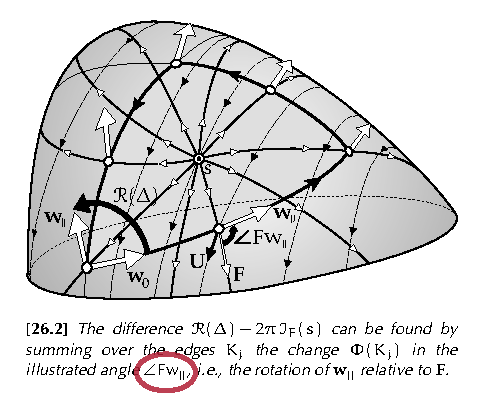
\includegraphics[width=0.9\textwidth]{figs/needham_triangle_circ.pdf}
\caption{{Needham,~T. (2021) Visual Differential Geometry and Forms.}}
\end{figure}
\column{0.5\textwidth}
\vspace{-12pt}
\begin{itemize}
\item The classical proof is discrete-flavored.
\item ``\( \angle Fw_{||} \)'' looked a lot like a pathover.
\item Hopf's \( \Phi \) is defined on edges, not loops. We imitated that too.
\end{itemize}
\end{columns}
\end{frame}
